\scanpage{71}
\mspage{324}

\deleted{On doit donc \unsure{avoir}}

\unsure{Désormais} nous nous \unsure{bornons} aux autom.
(\inserted{\unsure{eff. ou}} extérieurs) de $\widehat{\Pi}_{0,3}$
qui \unsure{respectent} la str. à lacets, et \unsure{commutent} à
$\mathfrak S_3$ (extérieurement)
--- qui \unsure{correspondent} aux autom.
\inserted{(\unsure{eff. ou ext.})} de
$\widehat{\mathfrak S}_{0,3}^{+}$ qui \unsure{induisent}
l'identité sur $\mathfrak S_3$,
et \unsure{satisfont} a) ci-dessus. \deleted{Ils \illegible{1}}

Les \unsure{autom.} \uline{extérieurs} de cette nature
\unsure{correspondent} donc aux aut. effectifs $u$
\inserted{de $\widehat{\Pi}_{0,3}$}
qui \unsure{commutent} à $\sigma_\infty$, i.e. $u$
\inserted{de $\widehat{\mathfrak S}_{0,3}^{+}$} qui
\unsure{fixent} $\sigma_\infty$, et sont déterminés par un
$g\in\widehat{\Pi}_{0,3}$ satisfaisant (38), \uline{et} tel que
de plus il existe \inserted{$p\in\widehat{\mathbb Z}^{*}$ et}
$g_0\in\widehat{\Pi}_{0,3}$ satisfaisant
\[
(39)\qquad
u(\ell'_0)=\operatorname{int}(g_0)({\ell'_0}^{p})
\qquad\text{i.e.}\qquad
u(\ell_0)=\operatorname{int}(g_0)(\ell_0^{p})
\]
(\unsure{où|i.e.} $g_0$ est déterminé mod $L_0=\ell_0^{\widehat{\mathbb Z}}$
\unsure{\ldots}). Des calculs faits par ailleurs \unsure{montrent}
\inserted{alors} qu'on doit avoir
\[
(40)\qquad g=\sigma_\infty(g_0)\,\ell_1^{\gamma}\,\rho(g_0)^{-1}
\]
\margin{avec $\gamma\in\widehat{\mathbb Z}$ bien déterminé
(\unsure{indépendant} du choix de $g_0$)}
i.e.
\[
(41)\qquad
\deleted{\rho(g_0)}\,\sigma_\infty(g_0)^{-1}\,
\underbrace{g\rho(g_0)}_{\unsure{g_1}}\in L_1
=\unsure{\mathcal N|N|\mathrm{Norm}}_{\widehat{\Pi}_{0,3}}(L_1)
\]

\scanpage{72}

En effet, on a par \unsure{hyp.} sur $g_0$ (cf (39))
\[
(42)\qquad u(L_0)=\operatorname{int}(g_0)(L_0)
\]
\unsure{\deleted{d'où}|d'où}
\[
\begin{aligned}
&u\sigma_\infty(L_0)=u(L_1)\overset{40}{=}
  \operatorname{int}(g_1)(L_1)\\
&\Vert\quad(\text{car }u\sigma_\infty=\sigma_\infty u)\\
&\sigma_\infty u(L_0)\underset{(42)}{=}
 \sigma_\infty(\operatorname{int}(g_0)(L_0))
 =\operatorname{int}(\sigma_\infty(g_0))(\sigma_\infty(L_0))
 =\operatorname{int}(\sigma_\infty(g_0))(L_1)
\end{aligned}
\]
d'où
\[
\operatorname{int}(\sigma_\infty(g_0)^{-1}g_1)(L_1)\subset L_1
\]
donc
\[
\sigma_\infty(g_0)^{-1}\underbrace{g_1}_{g\rho(g_0)}
\in \mathcal N_{\widehat{\Pi}_{0,3}}(L_1)=L_1
\]
d'où
\[
\sigma_\infty(g_0)^{-1}\unsure{g_1|g}\rho(g_0)=\ell_1^\gamma
\qquad (\gamma\in\widehat{\mathbb Z})
\]
d'où (40). On notera, pour \unsure{y revenir}, que l'élément $g$
défini en termes d'un $g_0$ \inserted{et de $\gamma$} \margin{$\checkmark$}
ne dépend en effet que de $g_0$ mod $L_0$. \deleted{\illegible{1}}

\margin{\figure{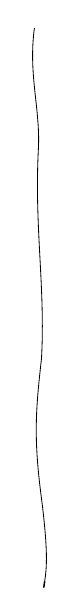
\begin{tikzpicture}[x=1cm,y=1cm,line cap=round]
\draw[line width=.30pt] (.03,0) .. controls (-.05,-.60) and (.11,-1.03) .. (.08,-1.55)
 .. controls (.03,-2.54) and (.17,-3.30) .. (.12,-4.20)
 .. controls (.04,-4.90) and (.02,-5.24) .. (.13,-6.05)
 .. controls (.20,-6.64) and (.19,-6.84) .. (.16,-7.03);
\draw[line width=.55pt] (.16,-7.03) -- (.15,-7.10);
\end{tikzpicture}}}
\unsure{Ainsi}; la donnée de $u_0$
\deleted{\unsure{satisfaisant à}} \inserted{\unsure{autom. ext.}}
à lacets de $\widehat{\Pi}_{0,3}$ \unsure{commutant} à
$\mathfrak S_3$, ou encore
\unsure{un|$u$} autom. ext. de $\widehat{\mathfrak S}_{0,3}^{+}$
\unsure{induisant} l'identité dans $\mathfrak S_3$
et \deleted{\unsure{transformant}}
\inserted{\unsure{laissant invariant}} la classe de conjugaison
du sous-groupe lacet
$L'_0=\varepsilon_0^{\widehat{\mathbb Z}}={\ell'_0}^{\widehat{\mathbb Z}}
=\widehat{\varphi}(L_0)$,
ou encore celle d'un autom. à lacets
$u_0$ de $\widehat{\Pi}_{0,3}$ \unsure{commutant} à
$\sigma_\infty$, et \unsure{ext.\textsuperscript{t}} à $\rho$,
ou encore d'un autom. $u$ de $\widehat{\mathfrak S}_{0,3}^{+}$
qui fixe $\sigma_\infty$, et qui fixe $\rho$ mod $\widehat{\Pi}_{0,3}$
--- \unsure{équivaut à} la donnée de $g_0\in\widehat{\Pi}_{0,3}$ mod $L_0$,
et de $\gamma\in\widehat{\mathbb Z}$, satisfaisant la relation

\scanpage{73}
\mspage{325}

\margin{\figure{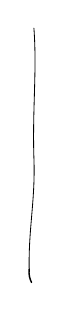
\begin{tikzpicture}[x=1cm,y=1cm,line cap=round]
\draw[line width=.30pt] (.04,0) .. controls (.08,-.55) and (.02,-1.02) .. (.04,-1.65)
 .. controls (.06,-2.18) and (-.03,-2.54) .. (-.02,-3.06);
\draw[line width=.52pt] (-.02,-3.06) .. controls (-.03,-3.13) and (-.01,-3.19) .. (.01,-3.23);
\end{tikzpicture}}}
\[
(38)\qquad \uline{g\rho(g)\rho^2(g)=1},
\]
où $g$ est donné par (40), et où $u$ s'exprime en termes de
\deleted{$g$} $g$ donc de $g_0,\gamma$ par
\[
(36)\qquad
\left\{\begin{aligned}
u(\sigma_\infty)&=\sigma_\infty\\
u(\rho)&=g\rho\qquad
\left(=\underbrace{\sigma_\infty(g_0)\ell_1^\gamma\rho(g_0)^{-1}}_g\rho\right).
\end{aligned}\right.
\]

\deleted{La relation (42)\inserted{\unsure{cf = ci-dessus}}, s'écrit alors,
comme $L_0$ est engendré par}
\[
\deleted{\ell_0=\underbrace{\ell'_0}_{\varepsilon_0}^{2}=(\sigma_\infty\rho)^2\deleted{\unsure{\sigma_\infty}}=\sigma_\infty\rho\sigma_\infty\rho}
\]
\[
\deleted{\underbrace{(u(\sigma_\infty\rho))}_{
\substack{\sigma_\infty g\rho=g_0\sigma_\infty \ell_1^\gamma\rho g_0^{-1}
=\operatorname{int}(g_0)(\sigma_\infty \ell_1^\gamma\rho)}}^{\unsure{2|4}}
\in\operatorname{int}(g_0)(\unsure{L'_0|L_0})\qquad\text{\unsure{or}}}
\]
\[
\deleted{\operatorname{int}(g_0)(\sigma_\infty \ell_1^\gamma\rho)^2\deleted{\unsure{g_0^{-1}}=1}}
\]
\deleted{donc (42) s'écrit}
\[
\deleted{(\sigma_\infty \ell_1^\gamma\rho)^2\in L_0}
\]
\deleted{\unsure{soit}}
\[
\deleted{
\underbrace{\sigma_\infty \ell_1^\gamma\sigma_\infty}_{
    \underbrace{\sigma_\infty(\ell_1)}_{\ell_0}^{\gamma}}
  \underbrace{\sigma_\infty\illegible{1}\rho}_{\varepsilon_0}
}
\]
\margin{\deleted{NB $\operatorname{int}(g_0^{-1})u(\ell_0)$}}
\margin{\deleted{NB on a
$(\operatorname{int}(g_0^{-1})u)(\ell_0)
=(\sigma_\infty \ell_1^\gamma\rho)^2=\ell_0^{2\gamma+1}$}}
\deleted{\unsure{soit}}
\[
\deleted{\overset{\varepsilon_0^{2\gamma+1}}{\unsure{\ell_0^\gamma}\ \underbrace{\varepsilon_0}_{\unsure{\varepsilon_0^{2\gamma}}}}\in L_0}
\]
\deleted{donc \unsure{\ldots}}
\[
\deleted{\unsure{\operatorname{int}(g_0)}\quad u(\ell_0)=}
\]

La relation (42), ou la relation \unsure{en apparence} plus forte
\[
(43)\qquad u(L'_0)\subset\operatorname{int}(g_0)(L'_0)
\]
s'écrit
\[
\underbrace{\operatorname{int}(g_0^{-1})\,
\underbrace{u(\underbrace{\sigma_\infty\rho}_{\ell'_0=\varepsilon_0})}_{
\sigma_\infty g\rho=g_0\sigma_\infty \ell_1^\gamma\rho g_0^{-1}}}_{
\sigma_\infty \ell_1^\gamma\rho
=\underbrace{\underbrace{\sigma_\infty \ell_1^\gamma\sigma_\infty}_{
 \underbrace{\sigma_\infty(\ell_1)^\gamma}_{\ell_0^\gamma=\varepsilon_0^{2\gamma}}}
\underbrace{\sigma_\infty\rho}_{\deleted{\unsure{\sigma_\infty\rho}}\varepsilon_0}}_{
\varepsilon_0^{2\gamma+1}}}
\in L'_0
\]
\margin{\uline{NB} on a
$\operatorname{int}(g_0^{-1})u(\underbrace{\ell'_0}_{\varepsilon_0})
=\varepsilon_0^{2\gamma+1}$}
\unsure{est vérifiée} automatiquement, on \unsure{aura}
$\overline{\mathrm m}$
\[
\deleted{(44)\qquad u(\ell'_0)=u(\varepsilon_0)
=\operatorname{int}(g_0)(\ell'}
\]

\scanpage{74}

\[
(44)\qquad
u\bigl(\underset{\substack{\Vert\\ \varepsilon_0}}{\ell'_0}\bigr)
 = \operatorname{int}(g_0)\bigl(\underset{\substack{\Vert\\ \varepsilon_0}}{\ell'_0}{}^{p}\bigr)
\qquad \text{avec}\quad \uuline{p=2\gamma+1}
\]
d'où (39), \deleted{d'où} en \unsure{élevant} au carré :
\[
u(\ell_0)=\operatorname{int}(g_0)(\ell_0^p).
\]

\deleted{\unsure{On}}\quad
\uline{NB} On \unsure{notera} que si $p\in\widehat{\mathbb Z}^{*}$, alors
$p-1\in 2\widehat{\mathbb Z}$ i.e.\ $\frac{p-1}{2}\in\widehat{\mathbb Z}$,
car il suffit de vérifier la relation analogue pour un $p\in\mathbb Z_\ell^{*}$,
\unsure{pour|que} $p-1\in 2\mathbb Z_\ell$, or si $\ell\ne2$ on a
$2\mathbb Z_\ell=\mathbb Z_\ell$ OK, \unsure{reste} le cas $\ell=2$
$p\in\mathbb Z_2^{*}$ donc l'image de $p$ dans $\mathbb Z/4\mathbb Z$
est $1$ ou $3$ donc $p-1\equiv0$ ou $2\bmod4$
\deleted{\illegible{3}} donc $\frac{p-1}{2}\in\mathbb Z_2$, OK.

\deleted{\unsure{Il reste donc à expri}}\par
Il reste donc à \unsure{exprimer} la condition (38), et on l'écrit
\deleted{\unsure{sous la forme}}
\[
\underbrace{\sigma_\infty(g_0)\ell_1^\gamma\rho(g_0^{-1})}\,
\underbrace{\rho\sigma_\infty(g_0)\ell_\infty^\gamma\rho^2(g_0^{-1})}\,
\rho^2\sigma_\infty(g_0)\ell_0^\gamma g_0^{-1}=1
\]
soit, en appliquant $\operatorname{int}(g_0^{-1})$ et
\deleted{\illegible{2}}\inserted{\unsure{posant encore}}
(cf (8))
\[
(45)\qquad g_0^{-1}\sigma_\infty(g_0)=h_0^{-1}
\qquad\text{i.e.}\quad
h_0=\sigma_\infty(g_0)^{-1}g_0=[\sigma_\infty,g_0^{-1}]
\]
\[
h_0^{-1}\ell_1^\gamma\underbrace{\rho(h_0^{-1})\ell_\infty^\gamma}\,
\rho^2(h_0^{-1})\ell_0^\gamma=1
\]
ou encore, en appliquant $\operatorname{int}(\ell_0^\gamma)$
\[
(46)\qquad
\boxed{\underbrace{(\ell_0^\gamma h_0^{-1})}\cdot
\rho(\ell_0^\gamma h_0^{-1})\cdot\rho^2(\ell_0^\gamma h_0^{-1})=1}
\qquad\left(\text{où }\gamma=\frac{p-1}{2}\right)
\]
ce qui n'est autre que (10). Quant à la condition \unsure{(9)|(7)},
on voit qu'elle est \inserted{superflue, i.e.,} automatiquement vérifiée.

\scanpage{75}
\mspage{326}

Résumons :

\uline{Théorème} Un autom. ext.\ \inserted{\unsure{à lcts|à lacets}} de
$\widehat{\Pi}_{0,3}$ commutant à
$\mathfrak S_3$, se relève de façon unique comme autom.
du groupe \unsure{à lcts|à lacets} $\widehat{\Pi}_{0,3}$, commutant à
$\sigma_\infty$ (et commutant à $\rho$ mod autom.\ \unsure{intérieures|intérieurs}),
ou encore comme restriction d'un autom.\ $u$ de
$\widehat{\mathfrak S}_{0,3}^{+}$
qui fixe $\sigma_\infty$, \unsure{invarie} $\rho$ mod $\widehat{\Pi}_{0,3}$
(i.e.\ \inserted{fixe} $\dot\rho$ dans $\mathfrak S_3$),
et qui \unsure{invarie} la classe de conjugaison du s-groupe
\inserted{fermé} $L'_0$\inserted{$=\widehat\varphi(L_0)$}
\deleted{\illegible{3}} engendré par $\ell'_0=\varepsilon_0=\sigma_\infty\rho$.
(ou encore du sous-groupe \inserted{fermé} $L_0=(L'_0)^2$ engendré par $\ell_0$).
La donnée d'un tel $u$ équivaut à celle de son multiplicateur
$p\in\widehat{\mathbb Z}^{*}$, et d'un $g_0\in\widehat{\Pi}_{0,3}/L_0$
satisfaisant les conditions suivantes

 a) Posant
\[
(47)\qquad
\begin{cases}
h_0=\sigma_\infty(g_0)^{-1}g_0=[\sigma_\infty,g_0^{-1}]
   \quad(\in\widehat{\Pi}_{0,3})\\
\gamma=\dfrac{p-1}{2}\in\widehat{\mathbb Z}
\end{cases}
\]
on a la relation (46) ci-dessus (invariante par remplacement de $g_0$ par
$g_0\ell_0^\lambda$, $\lambda\in\widehat{\mathbb Z}$)
\[
(48)\qquad
\bigl(\underbrace{\ell_0^\gamma h_0^{-1}}_{\xi_0}\bigr)
\rho(\ell_0^\gamma h_0^{-1})\rho^2(\ell_0^\gamma h_0^{-1})=1
\]
\margin{i.e.\ $\xi_0\rho(\xi_0)
\rho^{\unsure{2}}(\xi_0)=1$ avec
$\xi_0=\ell_0^\gamma h_0^{-1}$}

 b) $\sigma_\infty$ et $g\rho$ engendrent \unsure{top.}
$\widehat{\mathfrak S}_{0,3}^{+}$,
où $g$ est donné en fonction de $g_0$ par 40
\[
[(40)]\qquad
g=\sigma_\infty(g_0)\ell_1^\gamma\rho(g_0)^{-1}
=\sigma_\infty(g_0\ell_0^\gamma)\rho(g_0^{-1})
\]
\margin{$\begin{aligned}
&=g_0(h_0^{-1}\ell_1^\gamma)\rho(g_0)^{-1}\\
&=(g_0\ell_0^{-\gamma})(\ell_0^\gamma h_0^{-1})
  (\rho(g_0\ell_0^{-\gamma}))^{-1}
\end{aligned}$}

\deleted{\illegible{3}}
(\uline{NB} la relation (46) équivaut à :
\inserted{$(g\rho)^3=1$ i.e.\ à}
\[
(38)\qquad g\rho(g)\rho^2(g)=1,
\]
exprimée directement en termes de $g_0$, $\gamma=\frac{p-1}{2}$),
avec les relations génératrices $\sigma_\infty^2=(g\rho)^3=1$.
\margin{(36)}L'autom.\ $u$ est donné en termes de $g_0$ et de $p$ par

\scanpage{76}

\[
[(36)]\qquad
\begin{cases}
u(\sigma_\infty)=\sigma_\infty\\
u(\rho)=g\rho
\end{cases}
\qquad\text{où }g\text{ donné par }[(40)])
\]

On aura alors
\[
(49)\qquad
\begin{cases}
u(\ell_0)=\operatorname{int}(g_0)\ell_0^p\\
u(\ell_1)=\operatorname{int}(g_1)\ell_1^p
 \inserted{{}=\operatorname{int}(\sigma_\infty(g_0))(\ell_1^p)}\\
u(\ell_\infty)=\operatorname{int}(g_\infty)(\ell_\infty^p)
\end{cases}
\]
\margin{$\begin{aligned}
g_1&=g\rho(g_0)=\sigma_\infty(g_0)\ell_1^\gamma\\
   &=\sigma_\infty(g_0\ell_0^\gamma)\\
g_\infty&=g\rho(g_1)=\deleted{\unsure{g}}g\rho(g)\rho^2(g_0)\\
   &=\rho^2(g^{-1}g_0)=\rho(g_0\ell_0^\gamma)h_0
\end{aligned}$}

\margin{cf \unsure{prop.} plus haut}
\deleted{
\uline{Corollaire} Pour que l'hom.\ \unsure{surj.} (18)
\[
\widehat\varphi:\widehat\Pi_{\unsure{0,3|3}}
\longrightarrow
\widehat{\mathfrak S}_{0,3}^{+}
\]
\deleted{\unsure{déf}} défini par
\[
\ell_0\longmapsto \ell'_0=\sigma_\infty\rho,\quad
\ell_1\longmapsto \ell'_1=\sigma_\infty,\quad
\ell_\infty\longmapsto \ell'_\infty=\rho^{-1},
\]
commute \inserted{extérieurement} à $u$, il f. et s.\ qu'on puisse
\unsure{trouver} $\beta\in\widehat{\mathbb Z}$ tel qu'on ait
\[
[(24)]\qquad
\varepsilon_1^{-\beta}h_0\varepsilon_0^\beta
=\sigma_\infty(\widehat\varphi(h_0))^{-1}\widehat\varphi(h_0)
\]
ou ce qui revient au $\overline{\mathrm m}$, qu'il existe
$\alpha\in\widehat{\mathbb Z}$ tel qu'on ait
\[
[(\unsure{30|38})]\qquad
\deleted{\unsure{h_0^{-1}}\ell_1^\gamma\rho
=\operatorname{int}(\varepsilon_0^\alpha\widehat\varphi(
\unsure{\rho^{-1}(h_0)|\rho^{-1}h_0)}))(\rho^p)}
\]
\deleted{$u(\rho)=\operatorname{int}($}
\[
h_0^{-1}\ell_1^\gamma\rho
=\operatorname{int}(\varepsilon_0^\alpha\widehat\varphi(
\unsure{\rho^{-1}(h_0)|\rho^{-1}h_0)}))(\rho^p)
\]
(où nécessairement $\alpha=\beta+\gamma$).
}
\margin{$\beta$ \unsure{resp.} $\alpha$ sont \unsure{uniquement} \unsure{déterminés}}

\scanpage{77}
\mspage{327}

\uline{\unsure{Scholie}} Dans le \unsure{th.}, \unsure{le} $g$ \inserted{$\in\widehat{\Pi}_{0,3}$} (qui \unsure{intervient} directement pour écrire $u$) s'exprime par l'intermédiaire du $g_0$ \inserted{$\in\widehat{\Pi}_{0,3}$} et $\gamma=\frac{p-1}{2}$, \deleted{\illegible{2}} ($g_0$ défini mod $L_0$) --- la condition (46) étant en fait une condition qui s'exprime directement en termes de $g_0$, ou mieux encore, en termes de
\[
(50)\qquad
\xi_{\unsure{\deleted{0}|0}}=\ell_0^\gamma h_0^{-1}\in\widehat{\Pi}_{0,3}
\quad\text{(d'où }h_0=\xi_{\unsure{\deleted{0}|0}}^{-1}\ell_0^\gamma\text{)}
\]
comme
\[
(\unsure{51})\qquad \xi\rho(\xi)\rho^2(\xi)=1,
\]
qui équivaut à
\[
(52)\qquad (\xi\rho)^3=1.
\]

Les solutions de l'équation (\unsure{51}), ou ce qui revient au $\overline{\mathrm m}$ de (52), \unsure{correspondent} aux scindages de \unsure{la|l'}\inserted{\unsure{sous-}}extension \inserted{de $\widehat{\mathfrak S}_{0,3}^{+}$} de $\mathbb Z/3\mathbb Z$ par $\widehat{\Pi}_{0,3}$, \unsure{engendrée} par $\rho\in\mathfrak S_3$, \deleted{\illegible{1}} i.e. aux éléments d'ordre 3 de $\widehat{\mathfrak S}_{0,3}^{+}$ au dessus de $\dot\rho$.
Sur l'ens de ces scindages resp. de ces éléments $\xi\rho$, $\widehat{\Pi}_{0,3}$ opère par autom. intérieurs :
\[
(53)\qquad
\mathrm{int}(\lambda)(\xi\rho)
=\lambda\xi\rho\lambda^{-1}
=\lambda\xi\rho\lambda^{-1}\rho^{-1}\rho
=(\lambda\xi\rho(\lambda)^{-1})\rho
\]
i.e. il opère sur l'ens des solutions de (\unsure{51}), par
\[
(54)\qquad {}^\lambda\xi=\lambda\xi\rho(\lambda)^{-1}
\]
\margin{\uline{NB} $\lambda\mapsto{}^\lambda\xi$ est injectif}

\scanpage{78}

Admettons (quitte à le vérifier par la suite) qu'il y a exactement \unsure{deux} classes de conjugaison : celle de $\xi_0=1$, correspondant au scindage tautologique, \deleted{\illegible{1}}\inserted{de} sorte que pour de tels $\xi$ on aura
\[
(55)\qquad \xi=\lambda\rho(\lambda)^{-1}
\qquad(\lambda\in\widehat{\Pi}_{0,3}),
\]
et d'autre part la classe de conjugaison du \unsure{rel$^{\mathrm t}$} d'ordre 3 $\sigma_\infty\rho^{-1}\sigma_\infty^{-1}=\sigma_\infty\rho^{-1}\sigma_\infty$ de $\dot\rho$, correspondant à
\[
\sigma_\infty\rho^{-1}\sigma_\infty=\xi_0\rho,\quad\text{avec}
\]
\[
\left\{\begin{aligned}
\xi_0&=\sigma_\infty\rho^{-1}\sigma_\infty\rho^{-1}
=\sigma_\infty\underbrace{(\rho^{-1}\sigma_\infty)}_{\varepsilon_0^{-1}}(\rho^{-1}\sigma_\infty)\sigma_\infty\\
&=\sigma_\infty\varepsilon_0^{-2}\deleted{\unsure{=}}\sigma_\infty
=\sigma_\infty(\ell_0^{-1})=\ell_1^{-1}
\end{aligned}\right.
\]
(et on a bien
\[
\ell_1^{-1}\rho(\ell_1^{-1})\rho^2(\ell_1^{-1})
=\ell_1^{-1}\ell_\infty^{-1}\ell_0^{-1}
=(\ell_0\ell_\infty\ell_1)^{-1}=1
\]
), Cette orbite correspond à des solutions de la forme \deleted{\illegible{1}}
\[
(56)\qquad \xi=\lambda\ell_0^{-1}\rho(\lambda)^{-1}
\qquad(\lambda\in\widehat{\Pi}_{0,3})
\]
[on \unsure{notera} que $\ell_0^{-1}$ et $\ell_1^{-1}$ sont sur la $\overline{\mathrm m}$ orbite
\[
\ell_1^{-1}=\deleted{\unsure{\ell_0\ell_1}\ \lambda\ell_1^{-1}\rho(\lambda)^{-1}}
\ell_0(\ell_0^{-1})\rho(\ell_0)^{-1}
\]
]

i.e. \deleted{$\ell_0=\rho(\lambda)\ell_1\lambda^{-1}$ \illegible{1} où $\lambda=\ell_\infty\ell_{\unsure{0}}$}

\deleted{Posons}
\deleted{\unsure{a)}}

A) Cas \deleted{\unsure{A}} où $\xi$ est de la forme (55), donc
\[
(\unsure{56|57})\qquad h_0=\rho(\lambda)\lambda^{-1}\ell_0^\gamma
\]

\scanpage{79}
\mspage{328}

Il reste donc à résoudre l'équation en $g_0$ (47)
\[
(58)\qquad
\sigma_\infty(g_0)^{-1}g_0
=\underbrace{\rho(\lambda)\lambda^{-1}\ell_0^\gamma}_{h_0}
\]
Pour \unsure{$\forall$|un} $h_0$ fixé, il y a au plus un seul $g_0$ qui satisfait à cette condition, et un tel $g_0$ existe \unsure{ssi} \deleted{$\sigma_\infty(h_0)h_0=1$}, ce qui s'écrit
\margin{\unsure{en utilisant} \unsure{que} $\widehat{\Pi}_{0,3}^{\sigma_\infty}=\{1\}$}
\[
(59)\qquad \sigma_\infty(h_0)\cdot h_0=1
\qquad\inserted{\text{ou encore }h_0\sigma_\infty(h_0)=1}
\]
\deleted{$\sigma_\infty(\rho(\lambda))\sigma_\infty(\lambda^{-1})\ell_1^\gamma\rho(\lambda)\lambda^{-1}\ell_0^\gamma=1$}

qui s'écrit aussi, en reprenant l'expression $h_0=\xi^{-1}\ell_0^\gamma$
\[
\deleted{(\unsure{60})}\qquad
\sigma_\infty(\xi)^{-1}\ell_1^\gamma\xi^{-1}\ell_0^\gamma=1
\qquad\text{i.e.}
\]
\[
(60)\qquad \sigma_\infty(\xi)=\ell_1^\gamma\cdot\xi^{-1}\cdot\ell_0^\gamma
\]

En résumé

\uline{Corollaire} Les $u$ qui ne changent pas la classe de \inserted{$\widehat{\Pi}_{0,3}$-}conjugaison de $\rho$ \deleted{sont} correspondent 1-1 aux systèmes $(\lambda,p)\in L_0\backslash\widehat{\Pi}_{0,3}\times\widehat{\mathbb Z}^{*}$, tels que --- posant $\xi=\lambda\rho(\lambda)^{-1}$, \inserted{$\gamma=\frac{p-1}{2}$,} on ait la relation (60).
On notera que pour $\lambda$ \unsure{donc} $\xi$ fixé, il existe au plus \uuline{un} $\gamma\in\widehat{\mathbb Z}$ tel que la relation (60) soit valable, donc $p$ est déterminé par $\lambda$, soumis à la condition \unsure{suppl.} que \inserted{l'élément} $2\gamma+1$ de $\widehat{\mathbb Z}$ soit dans $\widehat{\mathbb Z}^{*}$ (i.e. $\exists\gamma'\in\widehat{\mathbb Z}^{*}$ \unsure{avec} $2\gamma\gamma'+\gamma+\gamma'=0$)

\scanpage{80}

\uline{NB} Si $\lambda$ est remplacé par $\lambda'=\ell_0^\alpha\lambda$, $\xi=\lambda\rho(\lambda)^{-1}$ est remplacé par $\xi'=\ell_0^\alpha\cdot\xi\rho(\ell_0)^{-\alpha}$, et $h_0=\xi^{-1}\ell_0^\gamma$ est remplacé par $h'_0=\rho(\ell_0)^\alpha h_0\ell_0^{-\alpha}$, enfin $g_0$ est remplacé par $g'_0=g_0\ell_0^{-\alpha}$, OK. \unsure{!} (L'équation (60) pour $\xi$ \unsure{ou} pour $\xi'$ est équivalente)

Finalement, que $u$ change ou ne change pas la classe de $\widehat{\Pi}_{0,3}$-conj. de $\rho$, la démarche la plus claire pour déterminer les $u$ en question me semble celle-ci :

1$^\circ$) On choisit un $\xi$ \inserted{$\in\widehat{\Pi}_{0,3}$} satisfaisant l'équation
\[
(A)\qquad \xi\rho(\xi)\rho^2(\xi)=1
\]
(on le \unsure{prendra} soit sous la forme (55), soit sous la forme (56)\deleted{\unsure{)}} :
\[
(B)\qquad
\xi=\lambda\rho(\lambda)^{-1}
\quad\text{ou}\quad
\xi=\lambda\ell_0^{-1}\rho(\lambda)^{-1}
\quad\deleted{\unsure{\rbrace|\xi}},\quad\text{avec }\lambda\in\widehat{\Pi}_{0,3}
\]
)

2$^\circ$) On choisit $\gamma\in\widehat{\mathbb Z}$ tel que
\[
(C)\qquad \sigma_\infty(\xi)=\ell_1^\gamma\xi^{-1}\ell_0^\gamma
\]
\margin{ici, $\xi$ est \unsure{donc} donné en termes de $\lambda$ \unsure{par par|par} (B)}
ce qui détermine $\gamma$ de façon unique. On devra dans \unsure{1$^\circ$)|2$^\circ$)} se borner aux $\xi$ \inserted{(i.e. aux $\lambda$)} pour lesquels un tel $\gamma$ existe, et tel de plus que $p=2\gamma+1$ soit $\in\widehat{\mathbb Z}^{*}$.
